% Options for packages loaded elsewhere
\PassOptionsToPackage{unicode}{hyperref}
\PassOptionsToPackage{hyphens}{url}
\documentclass[
]{article}
\usepackage{xcolor}
\usepackage{amsmath,amssymb}
\setcounter{secnumdepth}{-\maxdimen} % remove section numbering
\usepackage{iftex}
\ifPDFTeX
  \usepackage[T1]{fontenc}
  \usepackage[utf8]{inputenc}
  \usepackage{textcomp} % provide euro and other symbols
\else % if luatex or xetex
  \usepackage{unicode-math} % this also loads fontspec
  \defaultfontfeatures{Scale=MatchLowercase}
  \defaultfontfeatures[\rmfamily]{Ligatures=TeX,Scale=1}
\fi
\usepackage{lmodern}
\ifPDFTeX\else
  % xetex/luatex font selection
\fi
% Use upquote if available, for straight quotes in verbatim environments
\IfFileExists{upquote.sty}{\usepackage{upquote}}{}
\IfFileExists{microtype.sty}{% use microtype if available
  \usepackage[]{microtype}
  \UseMicrotypeSet[protrusion]{basicmath} % disable protrusion for tt fonts
}{}
\makeatletter
\@ifundefined{KOMAClassName}{% if non-KOMA class
  \IfFileExists{parskip.sty}{%
    \usepackage{parskip}
  }{% else
    \setlength{\parindent}{0pt}
    \setlength{\parskip}{6pt plus 2pt minus 1pt}}
}{% if KOMA class
  \KOMAoptions{parskip=half}}
\makeatother
\usepackage{longtable,booktabs,array}
\newcounter{none} % for unnumbered tables
\usepackage{calc} % for calculating minipage widths
% Correct order of tables after \paragraph or \subparagraph
\usepackage{etoolbox}
\makeatletter
\patchcmd\longtable{\par}{\if@noskipsec\mbox{}\fi\par}{}{}
\makeatother
% Allow footnotes in longtable head/foot
\IfFileExists{footnotehyper.sty}{\usepackage{footnotehyper}}{\usepackage{footnote}}
\makesavenoteenv{longtable}
\usepackage{graphicx}
\makeatletter
\newsavebox\pandoc@box
\newcommand*\pandocbounded[1]{% scales image to fit in text height/width
  \sbox\pandoc@box{#1}%
  \Gscale@div\@tempa{\textheight}{\dimexpr\ht\pandoc@box+\dp\pandoc@box\relax}%
  \Gscale@div\@tempb{\linewidth}{\wd\pandoc@box}%
  \ifdim\@tempb\p@<\@tempa\p@\let\@tempa\@tempb\fi% select the smaller of both
  \ifdim\@tempa\p@<\p@\scalebox{\@tempa}{\usebox\pandoc@box}%
  \else\usebox{\pandoc@box}%
  \fi%
}
% Set default figure placement to htbp
\def\fps@figure{htbp}
\makeatother
\setlength{\emergencystretch}{3em} % prevent overfull lines
\providecommand{\tightlist}{%
  \setlength{\itemsep}{0pt}\setlength{\parskip}{0pt}}
\usepackage{bookmark}
\IfFileExists{xurl.sty}{\usepackage{xurl}}{} % add URL line breaks if available
\urlstyle{same}
\hypersetup{
  hidelinks,
  pdfcreator={LaTeX via pandoc}}

\author{}
\date{}

\begin{document}

\section{A Conceptual Framework for Vision-Assisted Risk-Aware
Evacuation Route Recommendation in Confined Indoor
Environments}\label{a-conceptual-framework-for-vision-assisted-risk-aware-evacuation-route-recommendation-in-confined-indoor-environments}

Nazrul Anwar Bin Ramli, Jastini Mohd Jamil, Izwan Nizal Mohd Shaharanee,
Ang Jin Sheng

Department of Decision Science, School of Quantitative Sciences,
Universiti Utara Malaysia, Sintok, Malaysia

\subsection{Abstract}\label{abstract}

Indoor evacuation route recommendation in confined environments should
not depend only on the shortest path. In a real building, the shortest
route may pass through a crowded corridor, a blocked area,
smoke-affected space, or an exit that is no longer suitable. Previous
studies have discussed indoor navigation, fire evacuation routing,
dynamic risk-aware path planning, crowd detection, crowd counting,
indoor localization, and decision-support systems. However, these areas
are still often developed separately. Routing studies may assume that
crowd and hazard information is already available, while vision-based
crowd studies may stop at monitoring or people counting without showing
how the detected crowd condition can change the recommended route.
Therefore, this paper proposes a conceptual framework for
vision-assisted risk-aware evacuation route recommendation in confined
indoor environments. The framework is organized into six layers: spatial
environment modelling, risk representation, crowd perception, route
planning, decision-support visualization, and feedback-based replanning.
A literature-based design science approach is used to develop the
framework, and scenario walkthroughs are used to demonstrate how the
framework responds to a high-risk corridor, a crowded exit, and a
dynamic blockage or crowd update. The framework treats crowd condition
as local density, converts crowd levels into route-cost input, and
supports route explanation by comparing distance, risk exposure, crowd
exposure, and total route cost. In short, the paper contributes a
practical framework that connects vision-assisted crowd perception with
risk-aware route planning and explainable decision support. It also
provides a foundation for later simulation-based evaluation, expert
validation, and empirical testing of vision-based crowd-density input.

\textbf{Keywords:} indoor evacuation; risk-aware routing; crowd density;
vision-assisted navigation; crowd perception; decision support;
conceptual framework

\subsection{1. Introduction}\label{introduction}

Indoor environments such as hospitals, campuses, shopping malls,
transport terminals, libraries, office buildings, factories, and event
halls are not simple movement spaces. They contain rooms, corridors,
walls, doors, lifts, staircases, exits, restricted areas, and temporary
obstacles. In normal situations, indoor navigation may only need to
guide a user from one point to another. In emergency or high-density
situations, the problem becomes more serious because the most direct
path may not be the safest path.

Most navigation systems are designed to find the shortest or fastest
route. This is useful when the environment is open, stable, and low
risk. In confined indoor environments, however, a route has to be judged
by more than distance. A corridor may be short but congested. An exit
may be near but blocked. A path may be physically walkable but exposed
to smoke, fire, low visibility, high crowd density, or other hazards. In
this kind of situation, a longer route can be more useful if it helps
people avoid risk and crowd pressure.

The challenge also changes over time. A route that is acceptable at the
beginning may become crowded or blocked later. Fire, smoke, congestion,
and human movement patterns can all change route suitability. Studies on
indoor fire evacuation and dynamic routing show that geometric
shortest-path assumptions are not enough when smoke, structural damage,
congestion, and accessibility constraints are considered (Kim et al.,
2026; Zhou et al., 2020). Crowd dynamics research also shows that
high-density pedestrian movement can produce bottlenecks, jamming, and
unsafe movement conditions (Helbing et al., 2000; Helbing \& Johansson,
2013).

At the same time, computer vision and deep learning methods now make it
possible to detect people, count pedestrians, and estimate crowd density
from image or video input. YOLO-based models can detect people in low-
to moderate-density scenes, while density-estimation methods can support
crowd counting when individuals are heavily occluded (Chen et al., 2025;
Gao et al., 2025; Yiğit, 2025). However, crowd detection alone does not
solve the evacuation route problem. If a system only counts people, it
remains a monitoring system. For decision support, the detected crowd
condition must be translated into route-cost information that can
influence the recommended path.

The research gap, therefore, is not simply the absence of crowd
detection or the absence of routing algorithms. Both areas already
exist. The gap is the weak connection between crowd perception, risk
representation, route-cost modelling, and explainable decision support.
A vision system may detect congestion, but if the result is not
connected to route planning, it does not improve the route
recommendation. A routing system may calculate a path, but if it does
not receive updated crowd and hazard information, it may recommend a
route that is no longer suitable.

Based on this gap, this paper proposes a conceptual framework for
vision-assisted risk-aware evacuation route recommendation in confined
indoor environments. The term ``vision-assisted'' is used because the
framework can support multiple visual sensing sources, including CCTV,
smartphone camera input, depth cameras, LiDAR-enabled devices, or
vision-based density-estimation methods. The framework is not presented
as a certified emergency evacuation system. It is proposed as a
design-science artifact and decision-support structure that can guide
simulation-based evaluation and later empirical validation.

To address this problem, the study reviews related work on indoor
evacuation routing, risk-aware path planning, crowd perception, indoor
positioning, and decision-support systems. It then identifies the design
requirements needed to connect vision-based crowd perception with
risk-aware indoor route recommendation. The main focus is to show how
crowd density and risk conditions can be converted into route-planning
input, and how the resulting route can be explained through distance,
risk exposure, crowd exposure, and total route cost. The framework logic
is demonstrated through scenario walkthroughs and supported by a
proposed validation plan for later empirical evaluation.

The remainder of this paper is organized as follows. Section 2 reviews
related literature. Section 3 describes the methodology. Section 4
presents the proposed conceptual framework. Section 5 explains the
process flow. Section 6 demonstrates the framework using scenario
walkthroughs. Section 7 presents the validation plan. Section 8
discusses contributions, implications, and limitations. Section 9
concludes the paper and outlines future work.

\subsection{2. Literature Review}\label{literature-review}

\subsubsection{2.1 Indoor Navigation and Evacuation
Routing}\label{indoor-navigation-and-evacuation-routing}

Indoor navigation refers to guiding users from one indoor location to
another using spatial information, route-planning algorithms, and
positioning or environmental data. Unlike outdoor navigation, indoor
navigation is difficult because Global Navigation Satellite System
signals are often weak, unstable, or unavailable inside buildings.
Indoor environments also contain many movement constraints, including
walls, rooms, corridors, stairs, lifts, exits, obstacles, and restricted
areas (Łukasik et al., 2024).

Indoor route planning is commonly represented using graph-based or
grid-based models. In a graph model, important locations are represented
as nodes and walkable connections are represented as edges. In a grid
model, a floor plan is divided into cells. Each cell may represent a
walkable area, wall, blocked area, risk area, crowd area, start point,
or exit. These representations allow routing algorithms to compute a
route across the indoor space.

Dijkstra and A* are common baseline algorithms for indoor route
planning. Dijkstra's algorithm can find the shortest path when edge
weights are non-negative. A* improves search efficiency by using a
heuristic function to guide the search toward a destination. In
evacuation studies, these algorithms are useful baselines because they
are widely understood and easy to compare (Kim et al., 2026; Zhou et
al., 2020).

However, route-planning performance depends strongly on how route cost
is defined. If route cost only represents distance, the algorithm may
select a short but unsafe path. Fire evacuation routing studies show
that route calculation should consider semantics such as fire location,
smoke distribution, path accessibility, and exit condition (Zhou et al.,
2020). Dynamic evacuation studies further show that smoke and crowd
congestion can produce irregular route-performance outcomes, meaning no
single shortest-path algorithm is universally best under all dynamic
conditions (Kim et al., 2026).

\subsubsection{2.2 Risk-Aware Path
Planning}\label{risk-aware-path-planning}

Risk-aware path planning extends route calculation by adding
safety-related factors to the cost function. Instead of treating all
walkable areas as equal, risk-aware routing assigns higher cost to areas
with greater hazard or movement difficulty. Risk factors may include
fire, smoke, crowd congestion, blocked corridors, structural damage, low
visibility, restricted areas, or inaccessible exits.

The key principle is that a route should be evaluated by its total
suitability rather than only by its distance. A route that avoids smoke,
congestion, or a blocked exit may be longer but safer. Therefore, a
route-cost model can combine distance, risk exposure, crowd exposure,
blockage penalty, and exit accessibility.

Dynamic evacuation research supports this direction. Kim et al.~(2026)
evaluated Dijkstra and A* under structural damage, smoke, and crowd
congestion conditions in a multi-level underground station simulation.
Under static structural damage, both algorithms produced identical
maximum evacuation times, but A* required much less computation time.
Under dynamic smoke and crowd congestion, performance varied by scenario
and disaster location. This finding supports the need to evaluate routes
under dynamic risk and crowd conditions rather than assuming one
algorithm is always best.

Other studies also support the movement from shortest path to risk-aware
routing. Three-dimensional indoor fire evacuation routing research shows
that fire-related semantics and path accessibility can improve route
safety compared with pure geometric routing (Zhou et al., 2020). Mobile
evacuation guidance research also shows that dynamic edge weights, such
as smoke density, fire proximity, and crowd congestion, can support
safer route recalculation (Mocanu et al., 2026).

\subsubsection{2.3 Crowd Density, Crowd Detection, and Crowd
Counting}\label{crowd-density-crowd-detection-and-crowd-counting}

Crowd information is important in confined indoor evacuation because
congestion affects movement speed, comfort, route capacity, and safety.
A crowd should not be defined only by the total number of people. Twenty
people in a large hall may not be crowded, but twenty people in a narrow
corridor may create congestion. Therefore, this paper operationalizes
crowd condition as local pedestrian density. In pedestrian and crowd
studies, density is commonly expressed as the number of pedestrians
within a given area, often in persons per square meter, and is used to
describe movement comfort, congestion, and safety risk (Fruin, 1971;
Helbing \& Johansson, 2013; Yin et al., 2019).

The basic density formula is:

\[
\text{Crowd density} =
\frac{\text{Number of people in zone}}{\text{Zone area }(m^2)}
\]

For a grid-based route-planning model, the formula can be interpreted
as:

\[
\text{Cell density} =
\frac{\text{Detected people assigned to cell}}{\text{Real-world cell area }(m^2)}
\]

For the proposed framework, crowd density can be categorized into
practical levels as shown in Table 1. These categories are not proposed
as a new crowd-safety standard. They are synthesized from pedestrian
level-of-service logic and crowd-risk literature, where lower densities
indicate freer movement, densities around 3-4 persons per square meter
are treated cautiously, and about 5 persons per square meter is often
discussed as a critical crowd-risk level (Fruin, 1971; Helbing \&
Johansson, 2013; Yin et al., 2019). The exact threshold may be adjusted
depending on building type, corridor width, camera placement, and safety
policy.

\textbf{Table 1. Working crowd-density categories for route-cost
scoring, synthesized from Fruin (1971), Helbing and Johansson (2013),
and Yin et al.~(2019)}

{\def\LTcaptype{none} % do not increment counter
\begin{longtable}[]{@{}
  >{\raggedright\arraybackslash}p{(\linewidth - 4\tabcolsep) * \real{0.3000}}
  >{\raggedleft\arraybackslash}p{(\linewidth - 4\tabcolsep) * \real{0.4000}}
  >{\raggedright\arraybackslash}p{(\linewidth - 4\tabcolsep) * \real{0.3000}}@{}}
\toprule\noalign{}
\begin{minipage}[b]{\linewidth}\raggedright
Crowd level
\end{minipage} & \begin{minipage}[b]{\linewidth}\raggedleft
Approximate density
\end{minipage} & \begin{minipage}[b]{\linewidth}\raggedright
Route-planning meaning
\end{minipage} \\
\midrule\noalign{}
\endhead
\bottomrule\noalign{}
\endlastfoot
Low & 0.5 to 1.5 persons/m2 & Movement is possible with limited
interference \\
Medium & 1.5 to 3 persons/m2 & Movement is affected and route cost
should increase \\
High & 3 to 4 persons/m2 & Congestion risk is significant \\
Critical & Above 4-5 persons/m2 & Area should be avoided when
alternatives exist \\
\end{longtable}
}

Crowd safety studies often warn that dense crowds above approximately
3-4 persons per square meter should be treated cautiously, and around 5
persons per square meter is commonly considered critical in crowd-risk
contexts (Yin et al., 2019). This does not mean that a single universal
threshold applies to every building. Rather, it supports the need to
model crowd density as a risk factor rather than treating all walkable
space equally.

Vision-based crowd perception can estimate this condition using several
methods. YOLO-based object detection is suitable when people are visible
as individual objects (Chen et al., 2025; Yiğit, 2025). However, YOLO
may undercount people in dense scenes because of occlusion, perspective
distortion, lighting variation, and overlapping bodies. Crowd-counting
surveys show that density-map estimation can be useful when individual
detection becomes difficult under high-density conditions (Gao et al.,
2025). Therefore, the proposed framework allows crowd perception to use
person detection, head detection, density-map estimation, tracking, or
hybrid methods.

The important contribution is not the detection model alone. For
evacuation route recommendation, the useful output is not merely
``people detected.'' The useful output is ``crowd density by zone'' or
``crowd score by route cell.'' This score can then be used by the route
planning layer.

\subsubsection{2.4 Indoor Positioning and User
Location}\label{indoor-positioning-and-user-location}

Indoor positioning refers to estimating the location of a user, device,
or object inside a building. It is not one sensor by itself. It is a
system function that can use different signals, such as Wi-Fi, Bluetooth
Low Energy beacons, Ultra-Wideband, inertial measurement units,
camera-based localization, LiDAR, visual landmarks, QR codes, or sensor
fusion methods.

Indoor positioning is relevant because a route recommendation system
must know the user's start location. However, indoor localization
remains challenging because GPS is unreliable indoors and no single
indoor positioning method is universally dominant (Łukasik et al.,
2024). Combining multiple data sources can improve accuracy, but it also
increases system complexity.

In the proposed framework, indoor positioning is treated as a supporting
layer rather than the central contribution. The framework only requires
a start location to be available, and this start location may come from
manual selection, staff input, a mobile device, an indoor positioning
module, or another localization approach. The paper therefore does not
claim to solve real-time indoor positioning. Its main contribution is
the framework connection between crowd perception, risk scoring, route
planning, and decision-support explanation.

\subsubsection{2.5 Crowd Dynamics and Evacuation
Behaviour}\label{crowd-dynamics-and-evacuation-behaviour}

Crowd movement is complex because pedestrians do not behave as
independent geometric points. Their movement is affected by density,
bottlenecks, local interactions, route choice, visibility, social
behaviour, and environmental constraints. Classic crowd-dynamics
research has shown that evacuation situations can produce jamming and
``faster-is-slower'' effects, where increased pushing or urgency may
reduce flow efficiency (Helbing et al., 2000). Later crowd and
evacuation dynamics reviews explain how pedestrian interactions and
self-organized movement patterns influence evacuation outcomes (Helbing
\& Johansson, 2013).

At the same time, modern discussions caution against simplistic
assumptions about panic and irrational crowd behaviour. Haghani and
Ronchi (2024) argue that the terminology and assumptions around panic,
herding, and irrationality should be interpreted carefully and supported
by empirical evidence. This is important for the present framework
because it should not claim to model full human psychology. Instead, it
treats crowd density as a measurable environmental condition that
affects route cost.

Agent-based and simulation-based evacuation studies are useful for
future evaluation because they can model multiple pedestrians,
bottlenecks, and emergent crowd patterns. However, validation remains
difficult due to limited empirical evacuation data and simplified
modelling assumptions. Therefore, the present paper uses scenario
walkthroughs for conceptual demonstration and proposes simulation-based
evaluation as future work.

\subsubsection{2.6 Decision Support and
Explainability}\label{decision-support-and-explainability}

A decision-support system should help users or decision-makers
understand a recommendation. In evacuation route recommendation, simply
outputting a path is not enough. A route may be longer than the shortest
path, and users may question why it was selected. Therefore, the system
should explain the trade-off between distance, risk, crowd exposure,
blockage, and exit accessibility.

An explainable decision-support interface can show the indoor map,
selected route, alternative routes, risk zones, crowd zones, blocked
paths, exits, and route metrics. These metrics may include route
distance, risk score, crowd score, total cost, computation time, and
reduction in risk compared with a shortest-path baseline. In simple
terms, the system should show why a route is recommended, not only
display the route result.

\subsubsection{2.7 Design Science and Conceptual Framework
Development}\label{design-science-and-conceptual-framework-development}

Design science research is suitable for studies that develop useful
artifacts such as models, methods, frameworks, or architectures (Hevner
et al., 2004). The Design Science Research Methodology includes problem
identification, objective definition, design and development,
demonstration, evaluation, and communication (Peffers et al., 2007).
This paper aligns with design science because it proposes a conceptual
artifact to address a practical problem: how to integrate vision-based
crowd perception with risk-aware indoor route recommendation.

The current paper focuses on framework design and scenario-based
demonstration. It does not claim full deployment or certified emergency
use. Later work should evaluate the framework through simulation, expert
review, and empirical testing.

\subsubsection{2.8 Research Gap Summary}\label{research-gap-summary}

The reviewed literature shows that indoor evacuation routing, risk-aware
path planning, crowd detection, density estimation, indoor positioning,
and decision-support systems have each received research attention.
However, these areas are commonly studied separately. Route-planning
studies often focus on algorithmic route computation, while crowd
perception studies often focus on detection accuracy or people counting.
Decision-support explanation is not always integrated with algorithmic
output.

The gap addressed by this paper is the lack of an integrated conceptual
framework that connects vision-based crowd perception to risk-aware
route-cost modelling and explainable evacuation route recommendation.
Table 2 summarizes this gap.

\textbf{Table 2. Literature comparison and identified gap}

{\def\LTcaptype{none} % do not increment counter
\begin{longtable}[]{@{}
  >{\raggedright\arraybackslash}p{(\linewidth - 4\tabcolsep) * \real{0.3333}}
  >{\raggedright\arraybackslash}p{(\linewidth - 4\tabcolsep) * \real{0.3333}}
  >{\raggedright\arraybackslash}p{(\linewidth - 4\tabcolsep) * \real{0.3333}}@{}}
\toprule\noalign{}
\begin{minipage}[b]{\linewidth}\raggedright
Research stream and supporting citation
\end{minipage} & \begin{minipage}[b]{\linewidth}\raggedright
Existing contribution
\end{minipage} & \begin{minipage}[b]{\linewidth}\raggedright
Limitation for this study
\end{minipage} \\
\midrule\noalign{}
\endhead
\bottomrule\noalign{}
\endlastfoot
Indoor navigation (Łukasik et al., 2024) & Provides route guidance and
graph/grid modelling & Often emphasizes distance or travel efficiency \\
Fire evacuation routing (Kim et al., 2026; Zhou et al., 2020; Mocanu et
al., 2026) & Considers smoke, fire, accessibility, and dynamic hazards &
May assume crowd/risk input is already available \\
Risk-aware path planning (Kim et al., 2026; Zhou et al., 2020;
Lopez-Carmona and Paricio Garcia, 2021) & Adds hazard and congestion
factors into route cost & Often focuses on algorithm output rather than
explanation \\
Crowd detection (Chen et al., 2025; Yiğit, 2025) & Detects or counts
people from visual input & Often stops at monitoring rather than route
recommendation \\
Density estimation (Gao et al., 2025; Yin et al., 2019) & Supports
counting under occlusion and high density & Requires mapping into zones
and route-cost scores \\
Indoor positioning (Łukasik et al., 2024) & Estimates user location in
indoor spaces & Remains difficult and may require multimodal sensing \\
Decision support (Lopez-Carmona and Paricio Garcia, 2021; Hevner et al.,
2004; Peffers et al., 2007) & Visualizes recommendations and supports
decisions & Needs live or updated risk/crowd input \\
Proposed framework (this study) & Integrates spatial, risk, crowd,
routing, visualization, and feedback layers & Requires future empirical
validation \\
\end{longtable}
}

\subsection{3. Research Methodology}\label{research-methodology}

This study adopts a literature-based design science research approach.
The output is a conceptual framework, and the framework is treated as a
design artifact. The purpose is to organize the main components needed
for vision-assisted risk-aware evacuation route recommendation in
confined indoor environments.

The methodology consists of four stages:

\begin{enumerate}
\def\labelenumi{\arabic{enumi}.}
\tightlist
\item
  \textbf{Problem identification.} The study begins from the problem
  that shortest-path routing may be unsuitable when indoor routes are
  affected by risk, crowd density, blockage, or dynamic conditions.
\item
  \textbf{Objective definition.} The objective is to integrate spatial
  modelling, risk representation, crowd perception, route planning,
  decision support, and feedback-based replanning.
\item
  \textbf{Framework design.} A six-layer conceptual framework is
  proposed, with each layer described through its role, input, process,
  and output.
\item
  \textbf{Scenario-based demonstration and validation planning.}
  Scenario walkthroughs are used to show the framework logic, followed
  by a proposed plan for expert review and simulation-based evaluation.
\end{enumerate}

\textbf{Table 3. Design science mapping}

{\def\LTcaptype{none} % do not increment counter
\begin{longtable}[]{@{}
  >{\raggedright\arraybackslash}p{(\linewidth - 2\tabcolsep) * \real{0.5000}}
  >{\raggedright\arraybackslash}p{(\linewidth - 2\tabcolsep) * \real{0.5000}}@{}}
\toprule\noalign{}
\begin{minipage}[b]{\linewidth}\raggedright
Design science stage
\end{minipage} & \begin{minipage}[b]{\linewidth}\raggedright
Application in this paper
\end{minipage} \\
\midrule\noalign{}
\endhead
\bottomrule\noalign{}
\endlastfoot
Problem identification & Shortest-path routing may be unsafe in crowded
or hazardous indoor spaces \\
Objective definition & Develop an integrated framework for
vision-assisted risk-aware route recommendation \\
Design and development & Propose six connected framework layers \\
Demonstration & Use scenario walkthroughs to show route-decision
logic \\
Evaluation & Propose expert review and simulation-based validation \\
Communication & Present the framework as a conceptual article \\
\end{longtable}
}

This paper is not a full systematic literature review. PRISMA guidance
may be used in future work if a formal systematic review is conducted
(Page et al., 2021). In the present study, the literature is used mainly
to support framework construction and to identify design requirements.

\subsection{4. Proposed Conceptual
Framework}\label{proposed-conceptual-framework}

\subsubsection{4.1 Framework Overview}\label{framework-overview}

The proposed framework is designed to connect visual crowd perception
with route recommendation. The detail layers that happen in the
framework are the Spatial Environment Layer, Risk Representation Layer,
Crowd Perception Layer, Route Planning Layer, Decision-Support and
Visualization Layer, and Feedback and Replanning Layer.

The spatial environment layer provides the indoor layout. The risk
representation layer assigns risk values to hazards and unsafe areas.
The crowd perception layer estimates crowd density from visual input.
The route planning layer combines distance, risk, crowd, blockage, and
exit information. The decision-support layer visualizes and explains the
route. Finally, the feedback and replanning layer updates the route when
new conditions are detected.

\textbf{Figure 1. Proposed vision-assisted risk-aware evacuation route
recommendation framework}

\begin{figure}
\centering
\pandocbounded{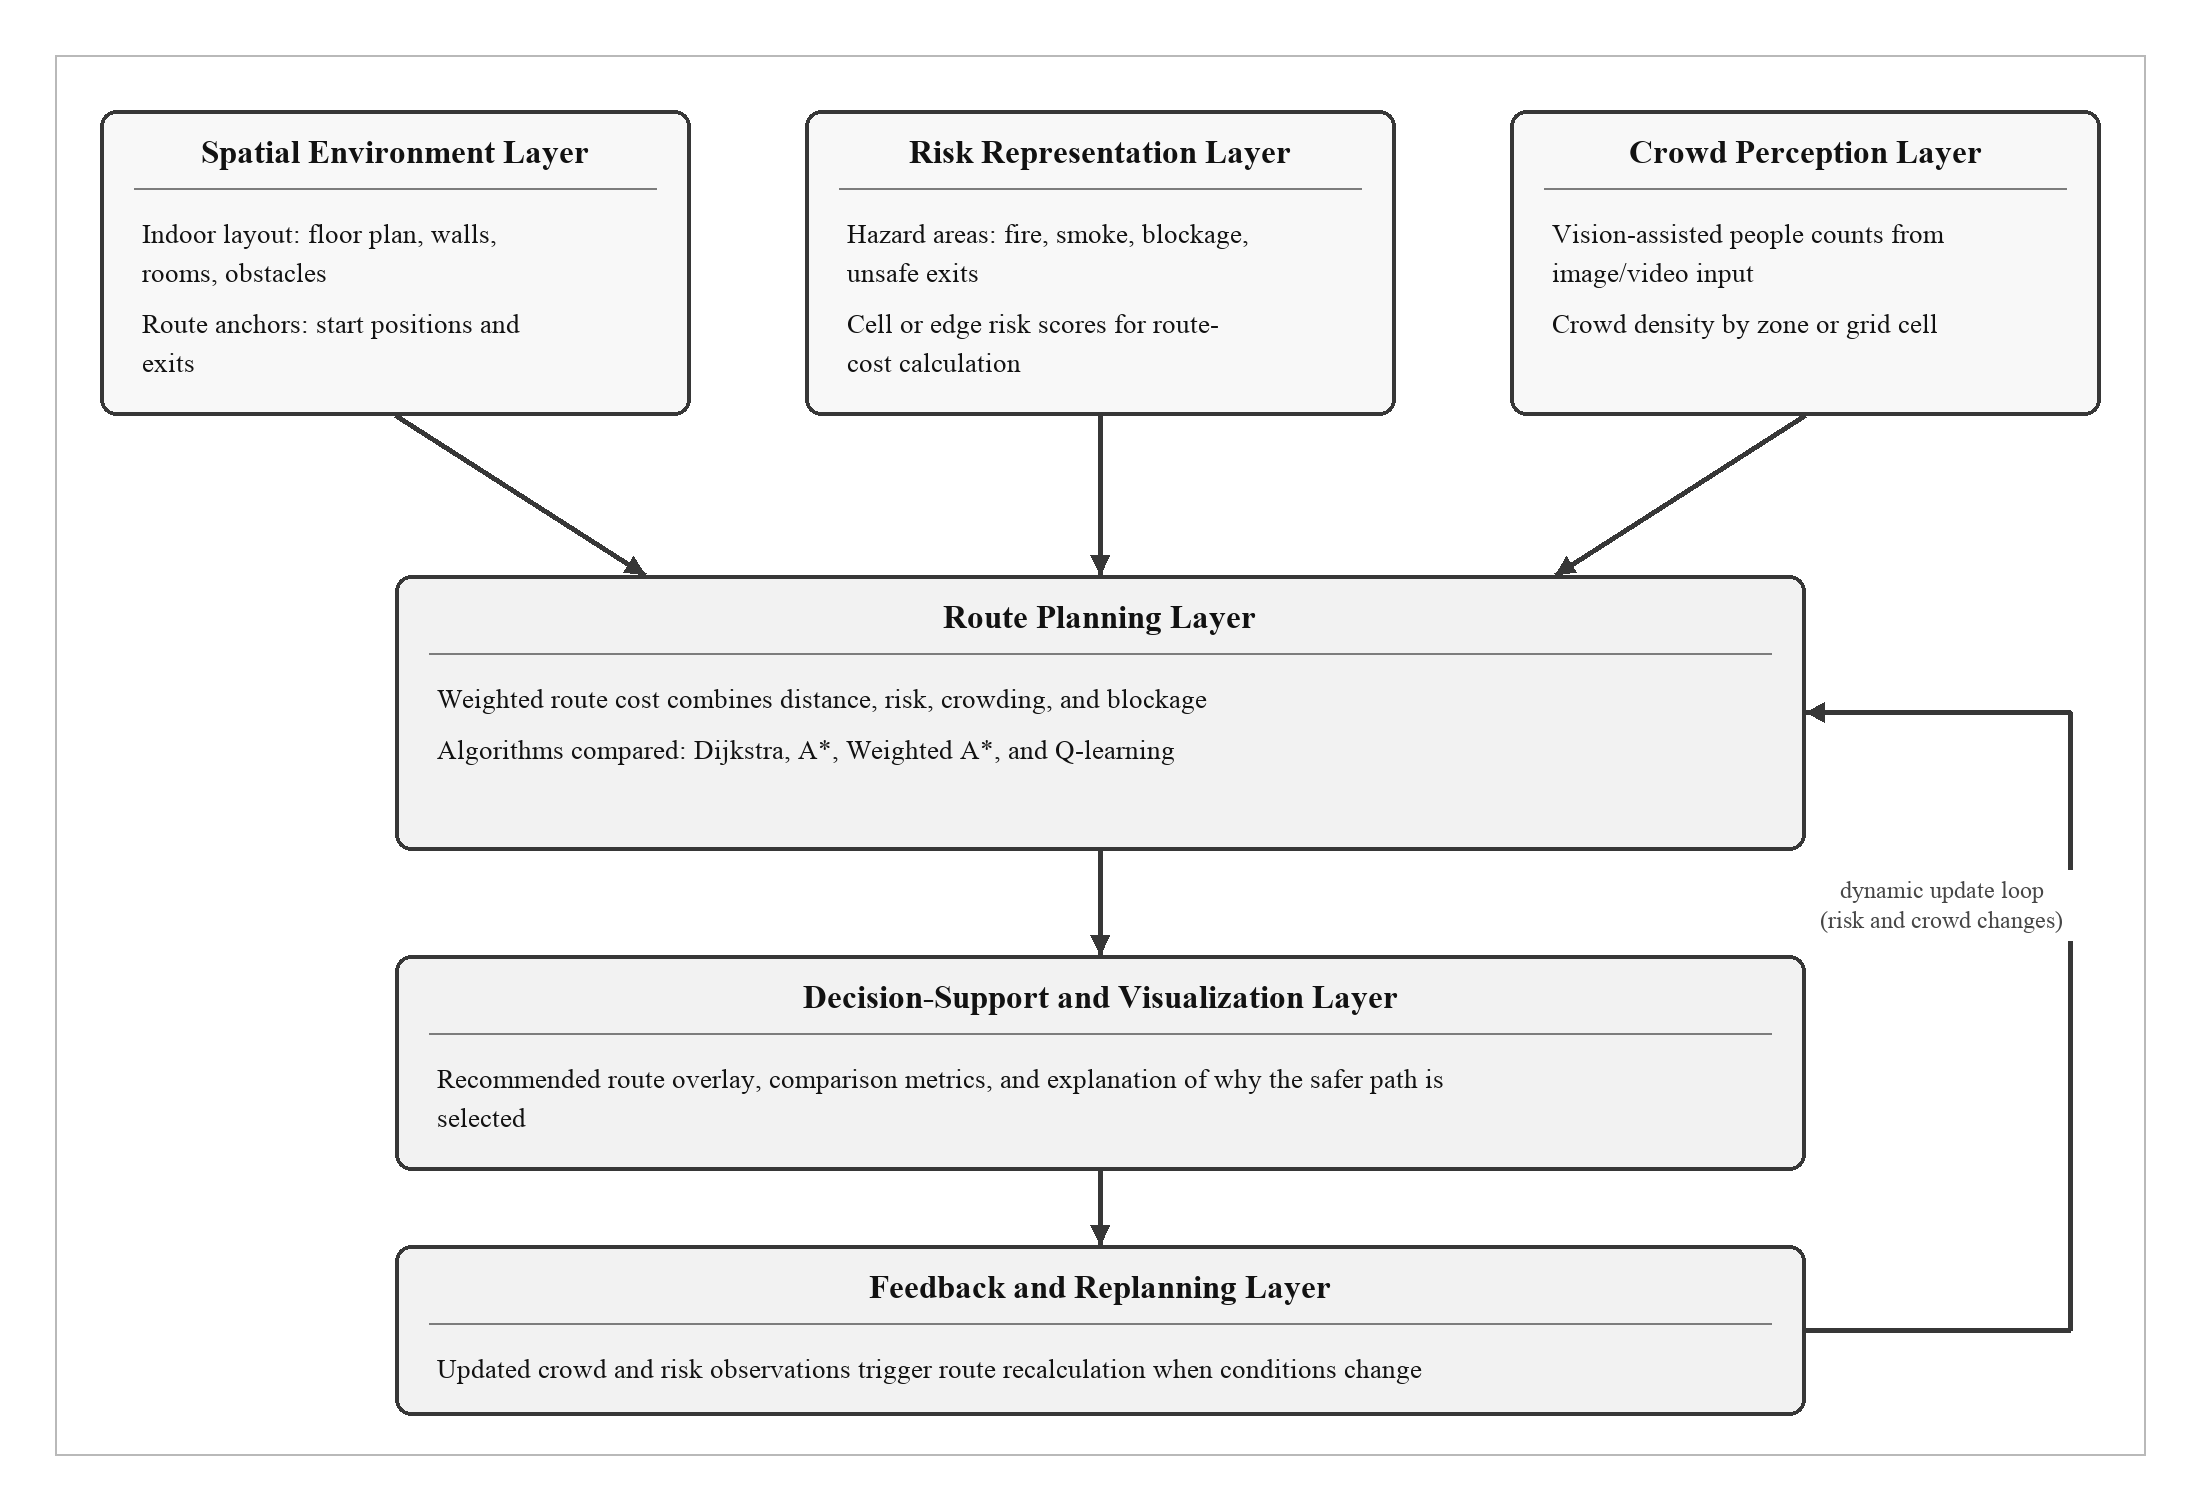
\includegraphics[keepaspectratio,alt={Proposed vision-assisted risk-aware evacuation route recommendation framework}]{../docs/assets/vision_assisted_framework_architecture.png}}
\caption{Proposed vision-assisted risk-aware evacuation route
recommendation framework}
\end{figure}

\subsubsection{4.2 Layer 1: Spatial Environment
Layer}\label{layer-1-spatial-environment-layer}

The spatial environment layer represents the physical indoor layout. It
includes corridors, rooms, walls, exits, staircases, lifts, doors,
obstacles, restricted areas, and blocked spaces. This layer can use a
floor plan, grid, graph, BIM model, or semantic indoor model.

For a grid-based implementation, each cell can be assigned a type, such
as empty, wall, blocked, risk, crowd, start, or exit. For a graph-based
implementation, locations can be represented as nodes and walkable links
as edges. The output of this layer is a structured route-planning model.

\subsubsection{4.3 Layer 2: Risk Representation
Layer}\label{layer-2-risk-representation-layer}

The risk representation layer converts hazards and unsafe conditions
into route-cost information. Risk may include fire, smoke, low
visibility, blocked corridors, structural damage, restricted zones, or
inaccessible exits. The risk score can be static or dynamic. For
example, a static score may be assigned manually from known floor-plan
information, while a dynamic score may be updated using sensor input,
staff reports, or simulation output.

The route planning layer uses this score to avoid high-risk areas when
alternatives exist. The intention is not to guarantee safety, but to
support better-informed route decisions compared with distance-only
routing.

\subsubsection{4.4 Layer 3: Crowd Perception
Layer}\label{layer-3-crowd-perception-layer}

The crowd perception layer estimates crowd condition from visual input.
Visual input may come from CCTV, fixed cameras, mobile phone cameras,
depth cameras, or future vision-based sensing systems. Depending on the
environment, the perception method may include:

\begin{itemize}
\tightlist
\item
  person detection using YOLO or similar object detectors;
\item
  head detection for partially occluded scenes;
\item
  density-map estimation for dense crowds;
\item
  tracking and temporal smoothing to reduce frame-level noise;
\item
  zone-based mapping from image regions to floor-plan areas.
\end{itemize}

The output is a crowd score or density level for each zone or route
cell. This score is then sent to the route planning layer. In this way,
visual crowd perception becomes useful for route recommendation, not
only for monitoring.

\subsubsection{4.5 Layer 4: Route Planning
Layer}\label{layer-4-route-planning-layer}

The route planning layer computes the recommended path using spatial,
risk, and crowd information. The route is not selected by distance
alone. Instead, route cost should include multiple factors:

\[
\text{Route cost} =
\text{Distance cost} + \text{Risk cost} + \text{Crowd cost}
+ \text{Blockage cost} + \text{Exit accessibility cost}
\]

At cell or edge level, a simplified weighted model can be expressed as:

\[
\text{Cell cost} =
\alpha(\text{Distance}) + \beta(\text{Crowd})
+ \gamma(\text{Risk}) + \delta(\text{Blockage})
\]

where alpha, beta, gamma, and delta are weights. Increasing the risk
weight makes the algorithm more likely to avoid hazardous areas.
Increasing the crowd weight makes the algorithm more likely to avoid
congested areas.

Dijkstra and A* can be used as shortest-path baselines. Weighted A* can
be used as an explainable risk-aware method because it can combine
heuristic search with weighted route costs. Learning-based methods, such
as reinforcement learning, may be explored in future work, but they
should be evaluated carefully rather than assumed to be better in every
situation.

\subsubsection{4.6 Layer 5: Decision-Support and Visualization
Layer}\label{layer-5-decision-support-and-visualization-layer}

The decision-support and visualization layer presents the recommendation
in an understandable form. It should show the indoor map, recommended
route, alternative route, start point, exits, risk zones, crowd zones,
and blocked areas. It should also show route metrics such as:

\begin{itemize}
\tightlist
\item
  distance;
\item
  risk exposure;
\item
  crowd exposure;
\item
  total route cost;
\item
  computation time;
\item
  reached exit;
\item
  risk reduction compared with a shortest-path baseline.
\end{itemize}

This layer is important because safer routes may be longer. If the
system recommends a longer route without explanation, users may not
trust it. If the system shows that the shorter route has higher risk or
crowd exposure, the recommendation becomes easier to understand and
justify.

\subsubsection{4.7 Layer 6: Feedback and Replanning
Layer}\label{layer-6-feedback-and-replanning-layer}

The feedback and replanning layer updates the route when conditions
change. New information may come from vision-based crowd detection, risk
sensors, manual reports, user input, or simulation. When a corridor
becomes crowded, an exit becomes blocked, or a risk zone changes, the
system updates the relevant crowd or risk score and recalculates the
route.

This feedback loop supports dynamic decision making. It also separates
the framework from static navigation systems that calculate one route
and assume the environment remains unchanged.

\subsubsection{4.8 Framework Layer
Summary}\label{framework-layer-summary}

\textbf{Table 4. Framework layer summary}

{\def\LTcaptype{none} % do not increment counter
\begin{longtable}[]{@{}
  >{\raggedright\arraybackslash}p{(\linewidth - 8\tabcolsep) * \real{0.2000}}
  >{\raggedright\arraybackslash}p{(\linewidth - 8\tabcolsep) * \real{0.2000}}
  >{\raggedright\arraybackslash}p{(\linewidth - 8\tabcolsep) * \real{0.2000}}
  >{\raggedright\arraybackslash}p{(\linewidth - 8\tabcolsep) * \real{0.2000}}
  >{\raggedright\arraybackslash}p{(\linewidth - 8\tabcolsep) * \real{0.2000}}@{}}
\toprule\noalign{}
\begin{minipage}[b]{\linewidth}\raggedright
Layer
\end{minipage} & \begin{minipage}[b]{\linewidth}\raggedright
Main function
\end{minipage} & \begin{minipage}[b]{\linewidth}\raggedright
Input
\end{minipage} & \begin{minipage}[b]{\linewidth}\raggedright
Process
\end{minipage} & \begin{minipage}[b]{\linewidth}\raggedright
Output
\end{minipage} \\
\midrule\noalign{}
\endhead
\bottomrule\noalign{}
\endlastfoot
Spatial environment & Represents indoor layout & Floor plan, walls,
corridors, exits & Convert layout into graph/grid/model & Indoor route
model \\
Risk representation & Represents hazards and unsafe areas & Fire, smoke,
blockage, restricted areas & Assign risk values to locations & Risk map
or score \\
Crowd perception & Estimates crowd level & Visual input from
camera/depth/CCTV/mobile device & Detection, counting, density
estimation & Crowd density or score \\
Route planning & Computes route recommendation & Map, risk, crowd,
start, destination & Weighted path planning & Recommended route \\
Decision support & Explains and visualizes recommendation & Route result
and metrics & Display route, scores, and explanation & Dashboard or
guidance interface \\
Feedback and replanning & Updates route when conditions change & New
crowd/risk/user data & Update scores and recalculate route & Revised
route recommendation \\
\end{longtable}
}

\subsection{5. Framework Process Flow}\label{framework-process-flow}

The framework can be described as a step-by-step process:

\begin{enumerate}
\def\labelenumi{\arabic{enumi}.}
\tightlist
\item
  \textbf{Indoor layout preparation.} The floor plan is converted into a
  route-planning model such as a grid or graph.
\item
  \textbf{Risk factor definition.} Risk zones, blocked areas,
  smoke-affected areas, or unavailable exits are assigned risk values.
\item
  \textbf{Crowd perception.} Visual input is processed to estimate
  people count or density by zone.
\item
  \textbf{Crowd-risk scoring.} Crowd density is converted into low,
  medium, high, or critical crowd scores.
\item
  \textbf{Route-cost calculation.} Distance, risk, crowd, blockage, and
  exit accessibility are combined into a weighted route cost.
\item
  \textbf{Route recommendation.} A route-planning algorithm recommends
  the lowest-cost route.
\item
  \textbf{Decision-support visualization.} The route, alternatives,
  risk/crowd zones, and explanation are displayed.
\item
  \textbf{Feedback and replanning.} Updated crowd or risk information
  triggers route recalculation when needed.
\end{enumerate}

\textbf{Table 5. Process flow summary}

{\def\LTcaptype{none} % do not increment counter
\begin{longtable}[]{@{}
  >{\raggedright\arraybackslash}p{(\linewidth - 4\tabcolsep) * \real{0.3333}}
  >{\raggedright\arraybackslash}p{(\linewidth - 4\tabcolsep) * \real{0.3333}}
  >{\raggedright\arraybackslash}p{(\linewidth - 4\tabcolsep) * \real{0.3333}}@{}}
\toprule\noalign{}
\begin{minipage}[b]{\linewidth}\raggedright
Step
\end{minipage} & \begin{minipage}[b]{\linewidth}\raggedright
Process
\end{minipage} & \begin{minipage}[b]{\linewidth}\raggedright
Description
\end{minipage} \\
\midrule\noalign{}
\endhead
\bottomrule\noalign{}
\endlastfoot
1 & Layout preparation & Convert floor plan into map, grid, graph, or
semantic model \\
2 & Risk definition & Assign risk scores to hazards and blocked areas \\
3 & Crowd perception & Detect people or estimate density from visual
input \\
4 & Crowd-risk scoring & Convert density into route-cost categories \\
5 & Route calculation & Compute route using weighted cost \\
6 & Visualization & Display route, metrics, and explanation \\
7 & Replanning & Update route when conditions change \\
\end{longtable}
}

\subsection{6. Scenario Walkthrough}\label{scenario-walkthrough}

Scenario walkthroughs are used to demonstrate the framework logic. They
do not represent final empirical validation. Their purpose is to show,
in a simple way, how the framework responds to different indoor
conditions.

\subsubsection{6.1 Scenario 1: Shortest Path Through a Risk
Zone}\label{scenario-1-shortest-path-through-a-risk-zone}

A user starts from Room A and needs to reach an exit. Two possible
routes are available. Route A is shorter but passes through a high-risk
corridor. Route B is longer but avoids the risk zone.

A distance-only system would normally select Route A. In the proposed
framework, the risk representation layer assigns a higher risk value to
the corridor. The route planning layer then combines distance and risk
score. Although Route B is longer, it may have lower total cost because
it avoids the high-risk area. The system therefore recommends Route B
and explains that the shorter route has higher risk exposure.

\subsubsection{6.2 Scenario 2: Nearest Exit With High Crowd
Density}\label{scenario-2-nearest-exit-with-high-crowd-density}

A user has access to two exits. Exit 1 is closer, but visual input
detects high crowd density near Exit 1. Exit 2 is farther but less
crowded.

The crowd perception layer estimates density near Exit 1 and classifies
it as high. This value is converted into a crowd-risk score. The route
planning layer increases the cost of routes that pass through the
crowded exit area. The system may recommend Exit 2 because it reduces
crowd exposure. The decision-support layer then explains that the
nearest exit is avoided due to crowd density.

\subsubsection{6.3 Scenario 3: Dynamic Crowd or Blockage
Update}\label{scenario-3-dynamic-crowd-or-blockage-update}

The system initially recommends Route A because it has acceptable
distance, low risk, and low crowd exposure. Later, visual input detects
increasing congestion along Route A, or staff reports that part of Route
A is blocked.

The feedback and replanning layer updates the crowd or risk score. The
route planning layer recalculates the route. If Route A is no longer
suitable, the system recommends Route B. This scenario demonstrates the
main idea of the framework: route recommendation should adapt when
indoor conditions change.

\textbf{Table 6. Scenario walkthrough summary}

{\def\LTcaptype{none} % do not increment counter
\begin{longtable}[]{@{}
  >{\raggedright\arraybackslash}p{(\linewidth - 8\tabcolsep) * \real{0.2000}}
  >{\raggedright\arraybackslash}p{(\linewidth - 8\tabcolsep) * \real{0.2000}}
  >{\raggedright\arraybackslash}p{(\linewidth - 8\tabcolsep) * \real{0.2000}}
  >{\raggedright\arraybackslash}p{(\linewidth - 8\tabcolsep) * \real{0.2000}}
  >{\raggedright\arraybackslash}p{(\linewidth - 8\tabcolsep) * \real{0.2000}}@{}}
\toprule\noalign{}
\begin{minipage}[b]{\linewidth}\raggedright
Scenario
\end{minipage} & \begin{minipage}[b]{\linewidth}\raggedright
Condition
\end{minipage} & \begin{minipage}[b]{\linewidth}\raggedright
Distance-only decision
\end{minipage} & \begin{minipage}[b]{\linewidth}\raggedright
Framework decision
\end{minipage} & \begin{minipage}[b]{\linewidth}\raggedright
Explanation
\end{minipage} \\
\midrule\noalign{}
\endhead
\bottomrule\noalign{}
\endlastfoot
Risk zone & Shortest route passes through high-risk area & Select
shortest route & Select longer safer route & Risk score increases
corridor cost \\
Crowded exit & Nearest exit has high crowd density & Select nearest exit
& Recommend less crowded exit & Crowd score affects route cost \\
Dynamic update & Route becomes crowded or blocked & Continue original
route & Recalculate route & Feedback layer updates route conditions \\
\end{longtable}
}

\subsection{7. Proposed Validation Plan}\label{proposed-validation-plan}

Because this paper presents a conceptual framework, validation should be
conducted in stages. The first stage is expert review. The second stage
is simulation-based framework evaluation. The third stage is real-world
or semi-controlled empirical testing when the framework is ready for
field validation.

\subsubsection{7.1 Expert Review}\label{expert-review}

Expert review can evaluate whether the framework is clear, complete,
feasible, and useful. Experts may come from indoor navigation,
evacuation planning, computer vision, safety management, built
environment, or information systems. They can review the framework
diagram, layer descriptions, process flow, scenario walkthroughs, and
proposed metrics before the system is developed further.

\textbf{Table 7. Expert review checklist}

{\def\LTcaptype{none} % do not increment counter
\begin{longtable}[]{@{}
  >{\raggedright\arraybackslash}p{(\linewidth - 2\tabcolsep) * \real{0.5000}}
  >{\raggedright\arraybackslash}p{(\linewidth - 2\tabcolsep) * \real{0.5000}}@{}}
\toprule\noalign{}
\begin{minipage}[b]{\linewidth}\raggedright
Evaluation item
\end{minipage} & \begin{minipage}[b]{\linewidth}\raggedright
Review question
\end{minipage} \\
\midrule\noalign{}
\endhead
\bottomrule\noalign{}
\endlastfoot
Clarity & Are the layers and information flow easy to understand? \\
Completeness & Are important components missing from the framework? \\
Feasibility & Can the framework be implemented using current visual
sensing and routing technologies? \\
Usefulness & Can the framework support safer route recommendation? \\
Explainability & Does the framework explain why a route is
recommended? \\
Replanning & Is the feedback loop suitable for dynamic indoor
conditions? \\
Scope control & Does the framework avoid overclaiming certified
emergency performance? \\
\end{longtable}
}

\subsubsection{7.2 Simulation-Based Framework
Evaluation}\label{simulation-based-framework-evaluation}

Later evaluation can test the framework using controlled simulation
scenarios. A grid-based or graph-based indoor model can be used to
compare distance-only routing with risk-aware routing. Dijkstra and A*
can be used as shortest-path baselines. Weighted A* can be used as the
main explainable risk-aware method. Learning-based methods can be
evaluated as additional comparison methods, but the comparison should
focus on evidence rather than assumption.

\textbf{Table 8. Future quantitative evaluation metrics}

{\def\LTcaptype{none} % do not increment counter
\begin{longtable}[]{@{}
  >{\raggedright\arraybackslash}p{(\linewidth - 4\tabcolsep) * \real{0.3333}}
  >{\raggedright\arraybackslash}p{(\linewidth - 4\tabcolsep) * \real{0.3333}}
  >{\raggedright\arraybackslash}p{(\linewidth - 4\tabcolsep) * \real{0.3333}}@{}}
\toprule\noalign{}
\begin{minipage}[b]{\linewidth}\raggedright
Metric
\end{minipage} & \begin{minipage}[b]{\linewidth}\raggedright
Meaning
\end{minipage} & \begin{minipage}[b]{\linewidth}\raggedright
Preferred direction
\end{minipage} \\
\midrule\noalign{}
\endhead
\bottomrule\noalign{}
\endlastfoot
Route distance & Number of steps or travel length & Lower, if safety is
not reduced \\
Risk exposure score & Exposure to hazard or risk zones & Lower \\
Crowd exposure score & Exposure to crowded zones & Lower \\
Total route cost & Weighted route score & Lower \\
Computation time & Time needed to compute route & Lower \\
Route success rate & Whether the route reaches a valid exit & Higher \\
Delta distance vs Dijkstra & Additional distance compared with
shortest-path baseline & Context dependent \\
Delta risk vs Dijkstra & Risk difference compared with shortest-path
baseline & Lower \\
Risk reduction percentage & Reduction in risk compared with Dijkstra &
Higher \\
Crowd reduction percentage & Reduction in crowd exposure compared with
Dijkstra & Higher \\
Explanation clarity & Expert/user rating of route explanation &
Higher \\
\end{longtable}
}

\subsubsection{7.3 Vision-Based Crowd
Evaluation}\label{vision-based-crowd-evaluation}

The framework can accommodate visual input that updates crowd scores
automatically. YOLO-based person detection is suitable for low- to
moderate-density scenes, while head detection, density-map estimation,
or hybrid methods may be more suitable for dense scenes. Evaluation
should compare estimated crowd level against manual counts or annotated
data.

\subsection{8. Discussion}\label{discussion}

\subsubsection{8.1 Conceptual
Contribution}\label{conceptual-contribution}

The main contribution of this paper is the integration of six components
that are often discussed separately: spatial environment modelling, risk
representation, crowd perception, route planning, decision-support
visualization, and feedback-based replanning. The framework shows how
visual crowd information can become a route-planning input instead of
remaining only as a monitoring output.

This contribution is important because crowd condition is a dynamic risk
factor. A route that is suitable under low density may become unsuitable
when congestion increases. By converting crowd density into a crowd-risk
score, the framework gives the routing layer a practical way to reduce
crowd exposure.

\subsubsection{8.2 Practical Implications}\label{practical-implications}

The framework can guide the design of decision-support systems for
buildings such as campuses, malls, libraries, hospitals, event venues,
and transport terminals. The framework can represent a floor plan with
manually assigned risk and crowd zones, integrate visual crowd detection
as a crowd-input layer, and include indoor positioning as a supporting
source of user location when needed.

The framework can also support safety officers and building managers.
Instead of only displaying a path, the system can explain why the path
is recommended. For example, it can show that the selected route is
longer but reduces risk exposure by a certain percentage compared with
the Dijkstra shortest-path baseline. This type of explanation is
important when the recommended route is not the shortest route.

\subsubsection{8.3 Operationalization
Implications}\label{operationalization-implications}

The framework can be operationalized through staged evaluation:

\begin{enumerate}
\def\labelenumi{\arabic{enumi}.}
\tightlist
\item
  \textbf{Simulation phase.} Use a grid-based floor plan with manual
  risk and crowd scores.
\item
  \textbf{Vision phase.} Use visual input to estimate people count or
  crowd density by zone.
\item
  \textbf{Integration phase.} Convert detected crowd density into
  crowd-risk scores.
\item
  \textbf{Routing phase.} Compare Dijkstra, A\emph{, Weighted A}, and
  selected learning-based methods.
\item
  \textbf{Decision-support phase.} Show route metrics, route overlays,
  and explanation text.
\item
  \textbf{Localization phase.} Add indoor positioning or mobile-device
  location estimation if required.
\end{enumerate}

This staged approach keeps the framework realistic. It also allows each
component to be evaluated independently before any real deployment is
considered.

\subsubsection{8.4 Limitations}\label{limitations}

This paper has several limitations. First, the framework is conceptual
and has not yet been fully validated in a real building. Second,
scenario walkthroughs demonstrate the logic but do not provide empirical
proof of safety improvement. Third, visual crowd perception may be
affected by occlusion, perspective distortion, lighting variation,
privacy requirements, camera placement, and domain shift. Fourth, indoor
positioning is treated as a supporting component and is not solved in
this paper. Fifth, route recommendation should not be interpreted as
certified emergency evacuation instruction without proper safety
validation, regulatory review, and deployment testing.

Despite these limitations, the framework provides a useful foundation
for future evaluation and system design. It defines how crowd
perception, risk scoring, route planning, and explanation can be
connected in one decision-support structure.

\subsection{9. Conclusion and Future
Work}\label{conclusion-and-future-work}

In a nutshell, this paper proposed a conceptual framework for
vision-assisted risk-aware evacuation route recommendation in confined
indoor environments. The framework is motivated by the limitation of
shortest-path routing under conditions involving crowd density, hazards,
blocked corridors, smoke, and unsuitable exits. It integrates six
layers: spatial environment modelling, risk representation, crowd
perception, route planning, decision-support visualization, and
feedback-based replanning.

The proposed framework contributes by linking vision-based crowd
perception to risk-aware route-cost modelling and explainable route
recommendation. It operationalizes crowd condition as local density,
supports the conversion of crowd levels into route-cost scores, and
provides a structure for explaining why one route is recommended over
another.

For future work, the framework should be evaluated using
simulation-based scenarios and expert review. The evaluation should
compare Dijkstra, A\emph{, Weighted A}, and selected learning-based
methods under risk and crowd conditions. Evaluation should include
distance, risk exposure, crowd exposure, total cost, computation time,
success rate, risk reduction percentage, crowd reduction percentage, and
explanation clarity. Later studies can examine real visual crowd
detection, density-map estimation, indoor positioning, and expert/user
evaluation within the same framework structure.

\subsection{References}\label{references}

Chen, Z., Xie, X., Qiu, T., \& Yao, L. (2025). Dense-stream YOLOv8n: A
lightweight framework for real-time crowd monitoring in smart libraries.
\emph{Scientific Reports, 15}, Article 11618.
https://doi.org/10.1038/s41598-025-94659-x

Gao, G., Gao, J., Liu, Q., Wang, Q., et al.~(2025). A survey of deep
learning methods for density estimation and crowd counting.
\emph{Vicinagearth, 2}, Article 2.
https://doi.org/10.1007/s44336-024-00011-8

Haghani, M., \& Ronchi, E. (2024). Revisiting the paper ``Simulating
dynamical features of escape panic'': What have we learnt since then?
\emph{Collective Dynamics, 9}, 1-11.
https://doi.org/10.17815/CD.2024.168

Helbing, D., Farkas, I., \& Vicsek, T. (2000). Simulating dynamical
features of escape panic. \emph{Nature, 407}, 487-490.
https://doi.org/10.1038/35035023

Helbing, D., \& Johansson, A. (2013). Pedestrian, crowd, and evacuation
dynamics. arXiv:1309.1609. https://arxiv.org/abs/1309.1609

Fruin, J. J. (1971). \emph{Pedestrian planning and design}. Metropolitan
Association of Urban Designers and Environmental Planners.

Hevner, A. R., March, S. T., Park, J., \& Ram, S. (2004). Design science
in information systems research. \emph{MIS Quarterly, 28}(1), 75-105.

Kim, H., Haam, S., Yoo, M., \& Song, W. S. (2026). Algorithmic
evaluation of fire evacuation efficiency under dynamic crowd and smoke
conditions. \emph{Fire, 9}(1), Article 32.
https://doi.org/10.3390/fire9010032

Lopez-Carmona, M. A., \& Paricio Garcia, A. (2021). CellEVAC: An
adaptive guidance system for crowd evacuation through behavioral
optimization. \emph{Safety Science, 139}, Article 105215.
https://doi.org/10.1016/j.ssci.2021.105215

Łukasik, S., Szott, S., \& Leszczuk, M. (2024). Multimodal image-based
indoor localization with machine learning: A systematic review.
\emph{Sensors, 24}(18), Article 6051. https://doi.org/10.3390/s24186051

Mocanu, A., Avram, C., Radu, D., Sita, I. V., \& Astilean, A. (2026).
Assistive mobile application for fire emergency evacuation of visually
impaired people. \emph{Sensors, 26}(5), Article 1572.
https://doi.org/10.3390/s26051572

Page, M. J., McKenzie, J. E., Bossuyt, P. M., Boutron, I., Hoffmann, T.
C., Mulrow, C. D., et al.~(2021). The PRISMA 2020 statement: An updated
guideline for reporting systematic reviews. \emph{BMJ, 372}, n71.
https://doi.org/10.1136/bmj.n71

Peffers, K., Tuunanen, T., Rothenberger, M. A., \& Chatterjee, S.
(2007). A design science research methodology for information systems
research. \emph{Journal of Management Information Systems, 24}(3),
45-77. https://doi.org/10.2753/MIS0742-1222240302

Senanayake, G. P. D. P., Kieu, M., Zou, Y., \& Dirks, K. (2024).
Agent-based simulation for pedestrian evacuation: A systematic
literature review. \emph{International Journal of Disaster Risk
Reduction, 111}, Article 104705.
https://doi.org/10.1016/j.ijdrr.2024.104705

Yiğit, G. (2025). Crowd detection: Leveraging YOLO for human
recognition. \emph{Turkish Journal of Engineering, 9}(3), 571-577.
https://doi.org/10.31127/tuje.1627839

Yin, J., Zheng, X.-M., \& Tsaur, R.-C. (2019). Occurrence mechanism and
coping paths of accidents of highly aggregated tourist crowds based on
system dynamics. \emph{PLOS ONE, 14}(9), e0222389.
https://doi.org/10.1371/journal.pone.0222389

Zhou, Y., Pang, Y., Chen, F., \& Zhang, Y. (2020). Three-dimensional
indoor fire evacuation routing. \emph{ISPRS International Journal of
Geo-Information, 9}(10), Article 558.
https://doi.org/10.3390/ijgi9100558

\end{document}
